
\section*{Appendix A: MNIST With Captions}

\begin{figure}[!t]
\captionsetup[subfigure]{labelformat=empty}
\begin{center}
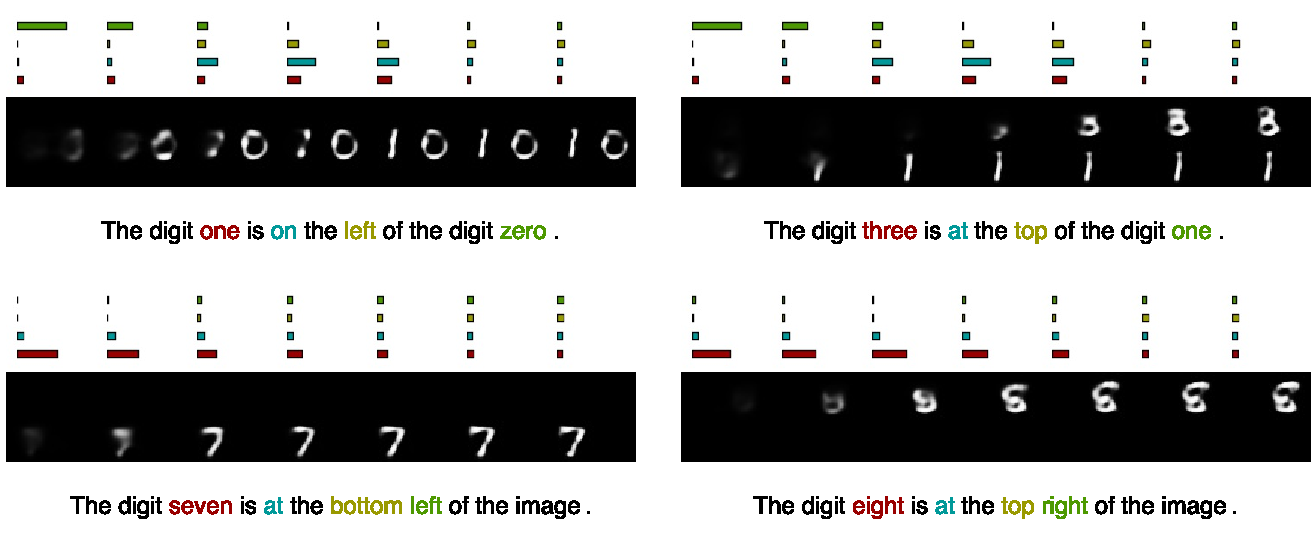
\includegraphics[width=0.99\textwidth]{figures/new/mnist/test3.pdf}\quad
%
\end{center}
\caption{Examples of generating $60 \times 60$ MNIST images corresponding to respective captions. The captions on the \textbf{left column} were part of the training set. The digits described in the captions on the \textbf{right column} were hidden during training for the respective configurations.}
\label{fig:figmnist}
\vspace{-0.3cm}
\end{figure}

As an additional experiment, we trained our model on the MNIST dataset with artificial captions. Either one or two digits from the MNIST training dataset were placed on a $60 \times 60$ blank image. One digit was placed in one of the four (top-left, top-right, bottom-left or bottom-right) corners of the image. Two digits were either placed horizontally or vertically in nonoverlapping fashion. The corresponding artificial captions specified the 
identity of each digit along with their relative positions, e.g. ``The digit two is on the top  
of the digit zero'', or ``The digit seven is at the bottom left of the image''.  

The generated images together with the attention alignments are displayed in Figure~\ref{fig:figmnist}. The model correctly displayed the specified digits at the described positions and even managed to generalize 
reasonably well to the configurations that were never present during training.
In the case of generating two digits, the model would dynamically attend 
to the digit in the caption it was drawing at that particular time-step. 
Similarly, in the setting where the caption specified only a single digit, the model would correctly 
attend to the digit in the caption during the whole generation process. 
In both cases, the model placed small attention values on the words describing the position of digits in the images.

\section*{Appendix B: Training Details}
\label{sec:training_details}

\subsection*{Hyperparameters}

Each parameter in alignDRAW was initialized by sampling from the Gaussian distribution with 
mean $0$ and standard deviation $0.01$. The model was trained using \textit{RMSprop} with initial learning rate of $0.001$. The norm of the gradients was clipped to $10.0$ during training to deal with exploding gradients. We used the vocabulary size of $K = 25323$ and $K = 22$ for Microsoft COCO and MNIST with Captions respectively. All capital letters in the words were changed to small letters to reduce the long tail. For all tasks, $\overrightarrow{h}^{lang}_{n}$ and $\overleftarrow{h}^{lang}_{n}$ in the language model had $128$ units. The parameters in \textit{align} operator had dimensionality of $l = 512$, $\vv \in \mathbb{R}^{512}$, $U \in \mathbb{R}^{512 \times 128}$, $W \in \mathbb{R}^{512 \times n^{gen}}$ and $b \in \mathbb{R}^{512}$. For the Microsoft COCO task, the alignDRAW model was trained for $18$ epochs and the learning rate was reduced by the factor of $0.1$ after $11$ epochs. The architectural configurations of alignDRAW models are shown on Table~\ref{tab:drawhyper}.

\begin{table}[!t]
\begin{center}
\begin{tabulary}{\linewidth}{c | c c c c c c}
\hline
\multicolumn{7}{c}{\textbf{alignDRAW Model}} \\
\hline
Task & \#glimpses & Inference \#$h$ & Generative \#$h$ & \#$z$ & Read Size & Write Size\\
\hline
Microsoft COCO & 32 & 550 & 550 & 275 & 9 & 9\\
MNIST Captions & 32 & 300 & 300 & 150 & 8 & 8\\
\end{tabulary}
\caption{The architectural configurations of alignDRAW models.}
\label{tab:drawhyper}
\end{center}
%\vspace{-0.3cm}
\end{table}

The GAN model used for sharpening had the same configuration as the $28 \times 28$ model trained by \cite{denton_lapgan} on the edge residuals of CIFAR dataset. The configuration can be found at \url{https://gist.github.com/soumith/e3f722173ea16c1ea0d9}. The model was trained for $6$ epochs.

\subsection*{Evaluation}

Table~\ref{tab:nll} shows the estimated variational lower bound on the average train/validation/test 
log-probabilities.
Note that the alignDRAW model does not suffer much from overfitting. 
The results worsened dramatically after sharpening test images.

\begin{table}[!h]
\begin{center}
\begin{tabulary}{\linewidth}{c | c c c c}
\hline
Model & Train LL & Valid LL & Test LL & Test LL (after sharpening)\\
\hline
skipthoughtDRAW & -1794.29 & -1797.41 & -1791.37 & -2045.84 \\
noalignDRAW & -1792.14 & -1796.94 & -1791.15 & -2051.07 \\
alignDRAW & -1792.15 & -1797.24 & -1791.53 & -2042.31
\end{tabulary}
\caption{The lower bound on the average test log-probabilities of conditional DRAW models, trained on the Microsoft COCO dataset.}
\label{tab:nll}
\end{center}
\end{table}

\newpage
\section*{Appendix C: Effect of Sharpening Images.}
\label{sec:post_processing}

\begin{figure}[!h]
\captionsetup[subfigure]{labelformat=empty}
\vspace{-0.27in}
\begin{center}
\subfloat[]{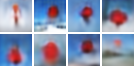
\includegraphics[width=0.23\textwidth]{figures/new/a-stop-sign-is-flying-in-blue-skies-blurry.png}}\quad
%
\subfloat[]{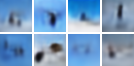
\includegraphics[width=0.23\textwidth]{figures/new/a-herd-of-elephants-flying-in-the-blue-skies-blurry.png}}\quad
%
\subfloat[]{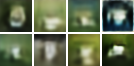
\includegraphics[width=0.23\textwidth]{figures/new/a-toilet-seat-sits-open-in-the-grass-field-blurry.png}}\quad
%
\subfloat[]{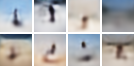
\includegraphics[width=0.23\textwidth]{figures/new/a-person-skiing-on-sand-clad-vast-desert-blurry.png}}\\
\vspace{-0.45cm}
%
\subfloat[%A stop sign is flying in blue skies.
]{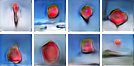
\includegraphics[width=0.23\textwidth]{figures/new/a-stop-sign-is-flying-in-blue-skies-sharp.png}}\quad
%
\subfloat[%A herd of elephants flying in the blue skies.
]{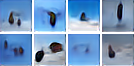
\includegraphics[width=0.23\textwidth]{figures/new/a-herd-of-elephants-flying-in-the-blue-skies-sharp.png}}\quad
%
\subfloat[%A toilet seat sits open in the grass field.
]{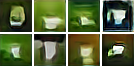
\includegraphics[width=0.23\textwidth]{figures/new/a-toilet-seat-sits-open-in-the-grass-field-sharp.png}}\quad
%
\subfloat[%A person skiing on sand clad vast desert.
]{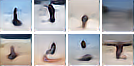
\includegraphics[width=0.23\textwidth]{figures/new/a-person-skiing-on-sand-clad-vast-desert-sharp.png}}\\
%

\subfloat[]{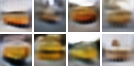
\includegraphics[width=0.23\textwidth]{figures/new/a-yellow-school-bus-parked-in-a-parking-lot-blurry.png}}\quad
%
\subfloat[]{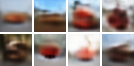
\includegraphics[width=0.23\textwidth]{figures/new/a-red-school-bus-parked-in-a-parking-lot-blurry.png}}\quad
%
\subfloat[]{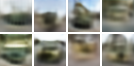
\includegraphics[width=0.23\textwidth]{figures/new/a-green-school-bus-parked-in-a-parking-lot-blurry.png}}\quad
%
\subfloat[]{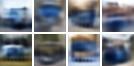
\includegraphics[width=0.23\textwidth]{figures/new/a-blue-school-bus-parked-in-a-parking-lot-blurry.png}}\\
\vspace{-0.45cm}
%
\subfloat[%A yellow school bus parked in a parking lot.
]{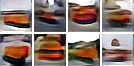
\includegraphics[width=0.23\textwidth]{figures/new/a-yellow-school-bus-parked-in-a-parking-lot-sharp.png}}\quad
%
\subfloat[%A red school bus parked in a parking lot.
]{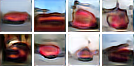
\includegraphics[width=0.23\textwidth]{figures/new/a-red-school-bus-parked-in-a-parking-lot-sharp.png}}\quad
%
\subfloat[%A green school bus parked in a parking lot.
]{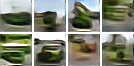
\includegraphics[width=0.23\textwidth]{figures/new/a-green-school-bus-parked-in-a-parking-lot-sharp.png}}\quad
%
\subfloat[%A blue school bus parked in a parking lot.
]{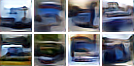
\includegraphics[width=0.23\textwidth]{figures/new/a-blue-school-bus-parked-in-a-parking-lot-sharp.png}}\\
%

\subfloat[]{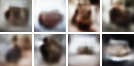
\includegraphics[width=0.23\textwidth]{figures/new/the-decadent-chocolate-dessert-is-on-the-table-blurry.png}}\quad
%
\subfloat[]{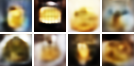
\includegraphics[width=0.23\textwidth]{figures/new/a-bowl-of-bananas-is-on-the-table-blurry.png}}\quad
%
\subfloat[]{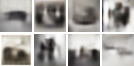
\includegraphics[width=0.23\textwidth]{figures/new/a-vintage-photo-of-a-cat-blurry.png}}\quad
%
\subfloat[]{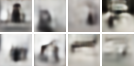
\includegraphics[width=0.23\textwidth]{figures/new/a-vintage-photo-of-a-dog-blurry.png}}\\
\vspace{-0.45cm}
%
\subfloat[%The decadent chocolate desert is on the table.
]{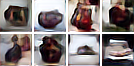
\includegraphics[width=0.23\textwidth]{figures/new/the-decadent-chocolate-dessert-is-on-the-table-sharp.png}}\quad
%
\subfloat[%A bowl of bananas is on the table.
]{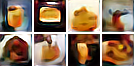
\includegraphics[width=0.23\textwidth]{figures/new/a-bowl-of-bananas-is-on-the-table-sharp.png}}\quad
%
\subfloat[%A vintage photo of a cat.
]{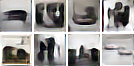
\includegraphics[width=0.23\textwidth]{figures/new/a-vintage-photo-of-a-cat-sharp.png}}\quad
%
\subfloat[%A vintage photo of a dog.
]{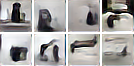
\includegraphics[width=0.23\textwidth]{figures/new/a-vintage-photo-of-a-dog-sharp.png}}\\
%

\subfloat[]{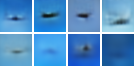
\includegraphics[width=0.23\textwidth]{figures/new/a-very-large-commercial-plane-flying-in-blue-skies-blurry.png}}\quad
%
\subfloat[]{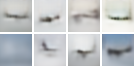
\includegraphics[width=0.23\textwidth]{figures/new/a-very-large-commercial-plane-flying-in-rainy-skies-blurry.png}}\quad
%
\subfloat[]{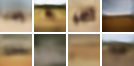
\includegraphics[width=0.23\textwidth]{figures/new/a-herd-of-elephants-walking-across-a-dry-grass-field-blurry.png}}\quad
%
\subfloat[]{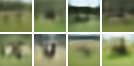
\includegraphics[width=0.23\textwidth]{figures/new/a-herd-of-elephants-walking-across-a-green-grass-field-blurry.png}}\\
\vspace{-0.45cm}
%
\subfloat[%A very large commercial plane flying in blue skies.
]{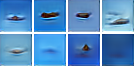
\includegraphics[width=0.23\textwidth]{figures/new/a-very-large-commercial-plane-flying-in-blue-skies-sharp.png}}\quad
%
\subfloat[%A very large commercial plane flying in rainy skies.
]{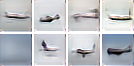
\includegraphics[width=0.23\textwidth]{figures/new/a-very-large-commercial-plane-flying-in-rainy-skies-sharp.png}}\quad
%
\subfloat[%A herd of elephants walking across a dry grass field.
]{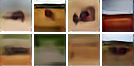
\includegraphics[width=0.23\textwidth]{figures/new/a-herd-of-elephants-walking-across-a-dry-grass-field-sharp.png}}\quad
%
\subfloat[%A herd of elephants walking across a green grass field.
]{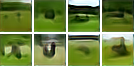
\includegraphics[width=0.23\textwidth]{figures/new/a-herd-of-elephants-walking-across-a-green-grass-field-sharp.png}}\\
%

\subfloat[]{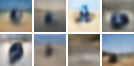
\includegraphics[width=0.23\textwidth]{figures/new/a-rider-on-a-blue-motorcycle-in-the-desert-blurry.png}}\quad
%
\subfloat[]{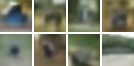
\includegraphics[width=0.23\textwidth]{figures/new/a-rider-on-a-blue-motorcycle-in-the-forest-blurry.png}}\quad
%
\subfloat[]{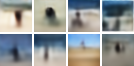
\includegraphics[width=0.23\textwidth]{figures/new/a-surfer-,-a-woman-,-and-a-child-walk-on-the-beach-blurry.png}}\quad
%
\subfloat[]{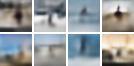
\includegraphics[width=0.23\textwidth]{figures/new/a-surfer-,-a-woman-,-and-a-child-walk-on-the-sun-blurry.png}}\\
\vspace{-0.45cm}
%
\subfloat[%A rider on a blue motorcycle in the desert.
]{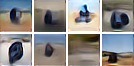
\includegraphics[width=0.23\textwidth]{figures/new/a-rider-on-a-blue-motorcycle-in-the-desert-sharp.png}}\quad
%
\subfloat[%A rider on a blue motorcycle in the forest.
]{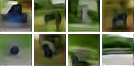
\includegraphics[width=0.23\textwidth]{figures/new/a-rider-on-a-blue-motorcycle-in-the-forest-sharp.png}}\quad
%
\subfloat[%A surfer, a woman, and a child walk on the beach.
]{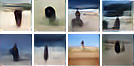
\includegraphics[width=0.23\textwidth]{figures/new/a-surfer-,-a-woman-,-and-a-child-walk-on-the-beach-sharp.png}}\quad
%
\subfloat[%A surfer, a woman, and a child walk on the sun.
]{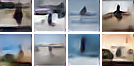
\includegraphics[width=0.23\textwidth]{figures/new/a-surfer-,-a-woman-,-and-a-child-walk-on-the-sun-sharp.png}}\\
\end{center}
%
%\caption{\small Effect of sharpening generated images shown in the publication \textbf{Bottom}: Sharpened Images. \textbf{Top}: Original Images}
%\vspace{-0.1in}
\end{figure}
